\chapter{工程和活动规划}
\label{chp:activity:begin}

\section{人体在不同条件下活动的能量消耗}
成年人的新陈代谢指数(取决于性别与体重):

Human Metabolic Rate Equation males > 19 years of age:
\begin{align*}
  & \left( \frac{622 - 9.53 \times age(years) + 1.25 \left(15.9 \times mass(kg) + 539.6 \times ht(m)\right)}{0.238853 \times 10^2} \right) \\
  &= Energy \frac{MJ}{CM-d}
\end{align*}

Human Metabolic Rate Equation females > 19 years of age:
\begin{align*}
  & \left( \frac{354-6.91 \times age(years) + 1.25 \left( 9.36 \times mass(kg) + 726 \times ht(m) \right)}{0.238853 \times 10^3} \right) \\
  &= Energy \frac{MJ}{CM-d}
\end{align*}

\begin{figure}[H]
  \centering
  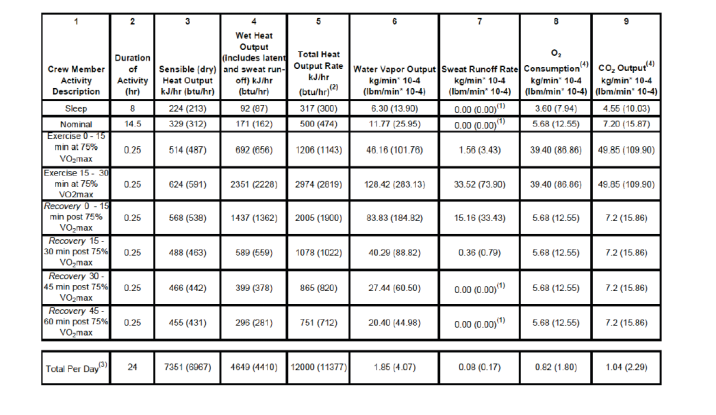
\includegraphics[width=\textwidth]{figure/metabolic.png}
  \caption{不同活动时常和所处环境下的能量消耗}
\end{figure}

\begin{figure}[H]
  \centering
  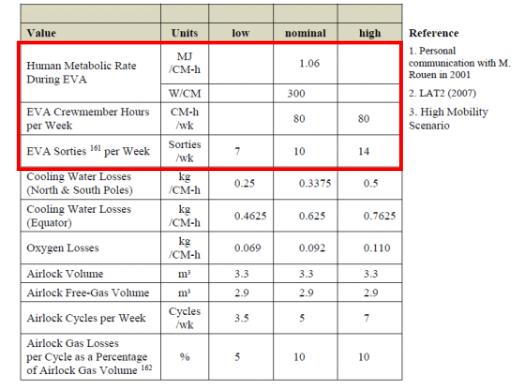
\includegraphics[width=0.8\textwidth]{figure/outdoor.png}
  \caption{舱外的活动数据}
\end{figure}

\begin{figure}[H]
  \centering
  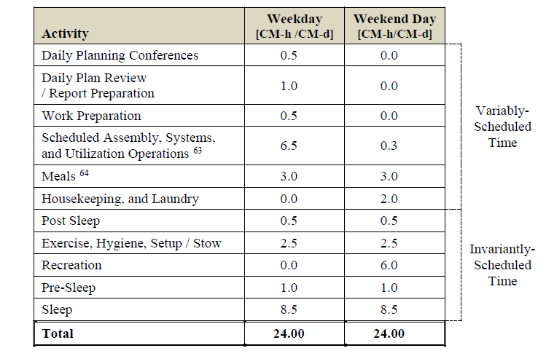
\includegraphics[width=0.8\textwidth]{figure/day-plan.png}
  \caption{一天的工作时间大致安排}
\end{figure}

结论:可以根据活动情况得到大致的能量消耗,并且给出了一个活动的时间模板。

\section{研究土壤转化}

\begin{figure}[H]
  \centering
  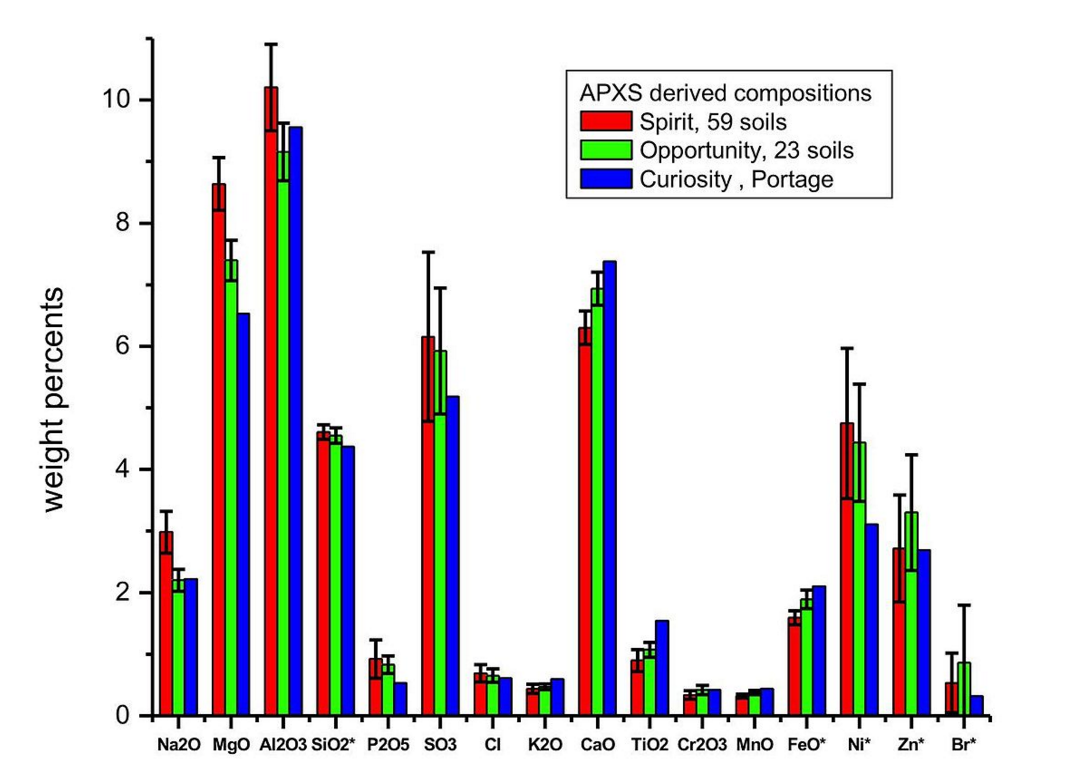
\includegraphics[width=0.8\textwidth]{figure/soil-composition.png}
  \caption{火星土壤成分比例}
\end{figure}
高氯酸盐的转化方法:

1.物理方法过滤:膜过滤和电渗析。

2.化学方法:(1)阴离子交换法(2)电化学还原法。
微生物转化方法:科研人员现已发现了多种厌氧微生物(正好火星上没氧气)可将高氯酸盐降解成无毒的氯酸盐和氧气。

降解机理:高氯酸盐和氯酸盐的还原过程如下所示:

高氯酸盐还原为氯酸盐和氯酸盐还原为亚氯酸盐的过程都是由高氯酸盐还原酶来催化完成的。亚氯酸盐被亚氯酸盐歧化酶歧化生成氧气和氯离子。由于高氯酸盐降解菌兼性厌氧的本性,不会在过程中积累。1\si{\mole}转化为1\si{\mole}需要8\si{\mole}电子,且需要细胞色素C作为电子传递体。

高氯酸盐降解菌在自然界中普遍存在,单菌多从含高氯酸盐的河流和土壤中分离得到。目前分离得到的56种高氯酸盐还原菌属于变形菌门种的α,β,γ和ε亚类。其中多数已知高氯酸盐降解菌属于β-变形菌纲,可利用硝酸盐、高氯酸盐、氯酸盐和作为电子受体。高氯酸盐降解菌多数属于红环菌目种的红环菌科,为菌属Dechloromonas和Dechlorosoma。

但目前已知的这些高氯酸降解菌仍然太过骄气,需在温度为10度到35度环境下才能正常进行降解工作。对环境要求较为严格,适用于火星的微生物需要经过严格筛选。

3.高温灭毒:高氯酸盐在高温下是强氧化剂,可用于火箭燃料。但这需要大量能源,而火星上能源缺乏。

结论:物理及化学方法需要较多的电力以及一些复杂的材料,操作过程也相对较为复杂。高温灭毒对于能源的要求过大。故微生物转化方法是最适合我们的方法,但是由于大部分微生物对生存环境的要求较高,需要根据火星的实际环境进行品种选择。

\section{辅助人类作业的工程机械}
有效载荷: 参考了两个过去的无人火星车的载荷配置:
\begin{figure}[H]
  \centering
  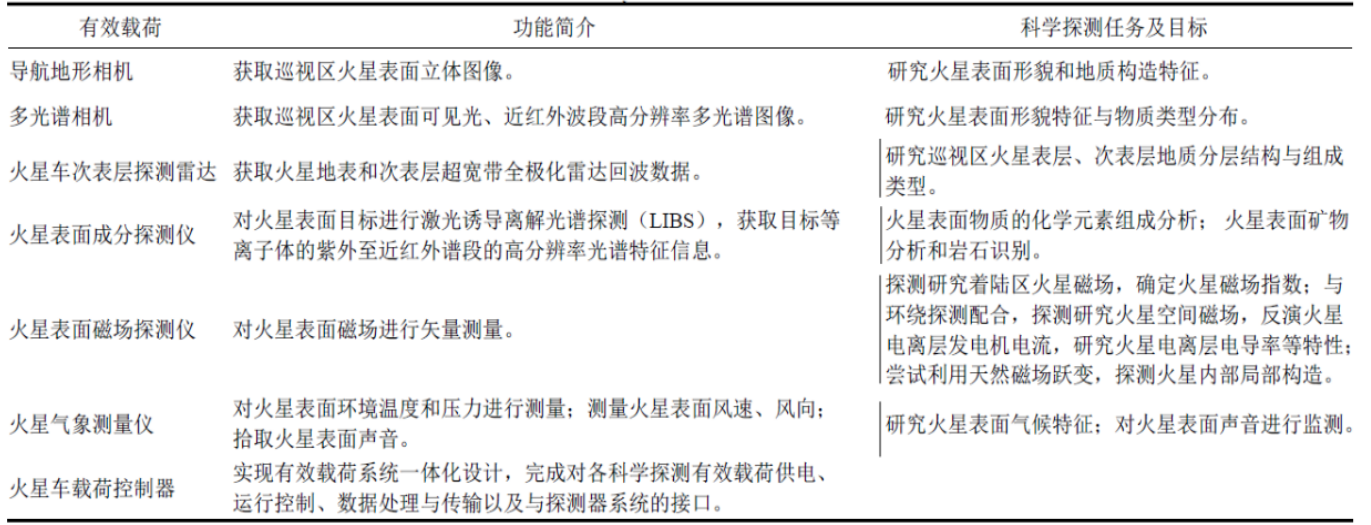
\includegraphics[width=\textwidth]{figure/effective-load.png}
  \caption{火星车有效载荷配置}
\end{figure}

俄罗斯福布斯探测器

1 等离子体-磁场探测系统(PhPMS):通过离子质谱仪对太阳风和行星粒子的分布进行探测;通过磁场探测器对变化的磁场进行探测。

2 掩星发射机。

3 微小粒子监视器(METEOR):用于研究微小粒子的物理动态参数,测量微小粒子的质量 速度及空间密度分布等。

4 土壤及气质普分析系统:由取土器、热分解器(TDA)、色谱分析器(GC)和质谱分析器(MS)等单机构成。科学目标是探测岩土内所含气体成分。测量土壤内水、二氧化碳、氮气、二氧化硫、惰性气体等化学物质和气体;探测土壤所含气体相态;探测土壤内所含有机物;探测元素碳、氢、氧、氮(13C/12C,D/H,17O/16O,18O/16O,15N/14N)和惰性元素的丰度;探测表面土壤所含矿物质成分。取土器安装在机械臂上,其余安装在内部。

5 GAMMA分析仪:用于分析表面岩石的主要化学组成(H-Fe)及放射性物质(K,Th,U)。

6 中子及γ射线分析仪:研究表面土层,用中子和γ射线分析有无与水相关的物质。

7 红外(IR)分析仪:探测甲烷、甲醛等物质;可探测高度60\si{\kilo\metre}的温度廓线;可绘制整体的矿物分布图;

8 次级离子质谱仪:对表面进行地质勘探。

9 长波雷达:探测深层结构,估算岩层厚度。

10 导航及引导系统:用于在靠近时进行导航,着陆地点选择,着陆时进行辅助控制、表面成像。

11 全景立体相机:获得着陆地点的全景图像,以及着陆时的实时3D成像。

12 红外显微镜:安装于机械臂2,帮助选择返回地球的采样土壤。

结论:主要需要其中的 导航系统、多种相机系统(普通高分辨率相机,全景立体相机,多光谱相机)、表面成分分析系统(土壤及气质普分析器)、气象测量仪、雷达系统、红外显微镜。

载人火星车的更多需求:
我们选用有可增压装置的载人车辆,可以作为移动居住舱,长时间进行生活或移动工作。
由于并没有载人火星车的应用历史,所以选择已有的载人月球车作为参考模板。

\begin{figure}[H]
  \centering
  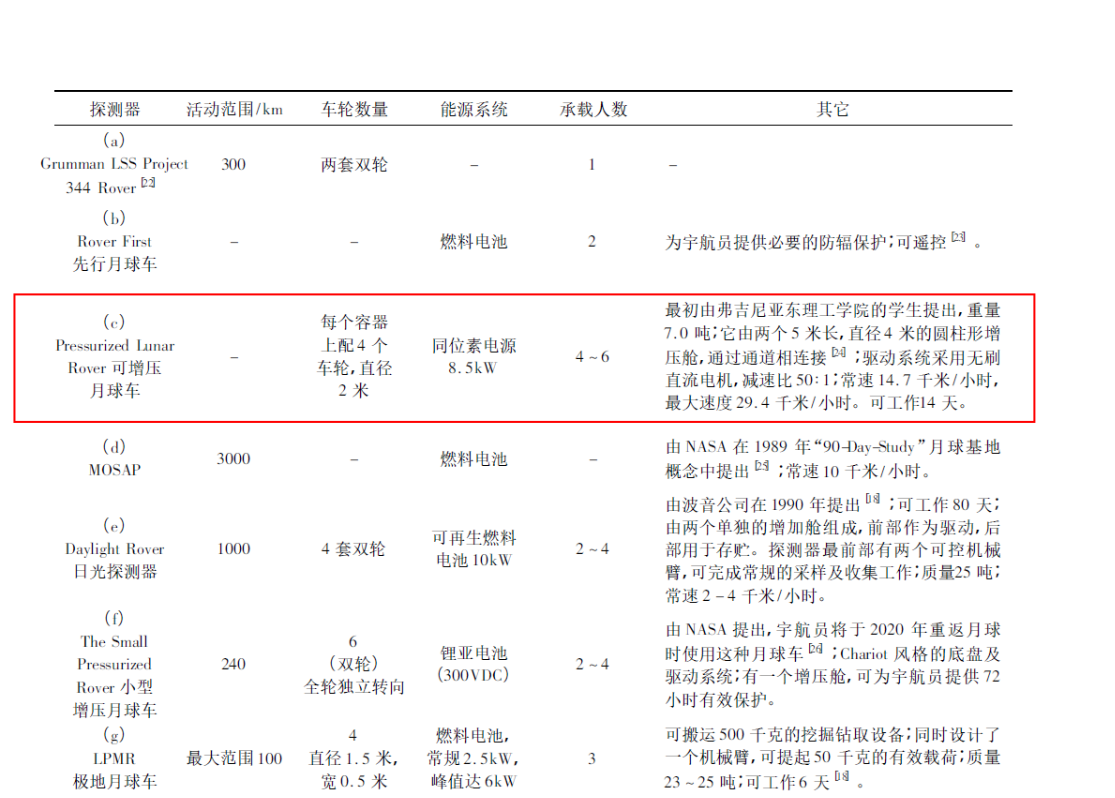
\includegraphics[width=\textwidth]{figure/moon-cart.png}
  \caption{有可增压装置的载人月球车}
\end{figure}

\begin{figure}[H]
  \label{chp:activity:end}
  \centering
  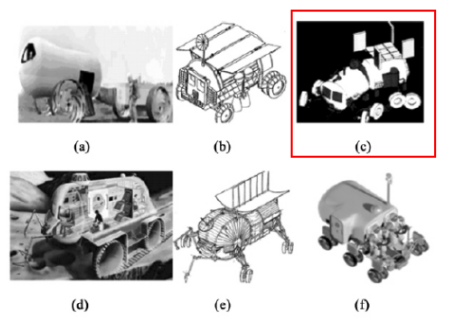
\includegraphics[width=0.8\textwidth]{figure/variety-cart.png}
  \caption{火星车的选择}
\end{figure}

结论:选择(c)型的月球车作为我们所需的载人火星车的参考模型。

并且得到了大致的火星车参数:

能源需求:8.5\si{\kilo\watt} 300\si{\volt}DC同位素电源。

续航情况:速度14.7--29.4\si{\kilo\metre\per\hour},正常使用情况下可续航14天左右。
